\subsection{Initial Contractual Refinement}
\label{sec:granularityANDAlg}
The simplest restructuring that could be done on the model was to split any guarantees containing an $\land$ at the highest level of the binary Boolean formula and create additional guarantees from this refinement. The analysis performed on the model treats all guarantees as a large conjunction. This enables one to automatically split guarantees with expressions containing at the top level a conjunctive operator into two separate expressions. For instance, if $g_0 = A \land B$, then split this into $g_1 = A$, and $g_2 = B$ and insert $g_1$ and $g_2$ into the model. This was an initial probing of a deeper issue and gave a preliminary look into our assumption regarding minimal cut set generation in a model similar to that described in Section~\ref{sec:granularityEx}. Algorithm~\ref{alg:splitAnd} shows this algorithm used in this investigation. 

\begin{algorithm}[h]
\SetKwFunction{FMain}{$splitOnAnd$}
 \SetKwProg{Fn}{Function}{:}{}

	\Fn{\FMain{expression}}{
		Program $P$ \;
		Guarantees $list_G$ \;
		\For{all $g \in list_G$}{
			\If{binary statement with operator $\land$}{
			    insert into $P$ $\rightarrow$ new guarantee (left) \;
			    insert into $P$ $\rightarrow$ new guarantee (right) \;
				\FMain(left) \;
				\FMain(right) \;
			} %end if there exists AND in G
		}%end for all g in P
	}
	\caption{Split guarantees on logical $\land$ operator}
	\label{alg:splitAnd}
\end{algorithm}

The sensor described in Section~\ref{sec:granularityEx} is encoded into Lustre originally had a single guarantee as shown in Figure~\ref{fig:lustreOneGuar} that contained two subexpressions -- one of which was unrelated to the proof of the safety property.
\begin{figure}[h!]
\begin{center}
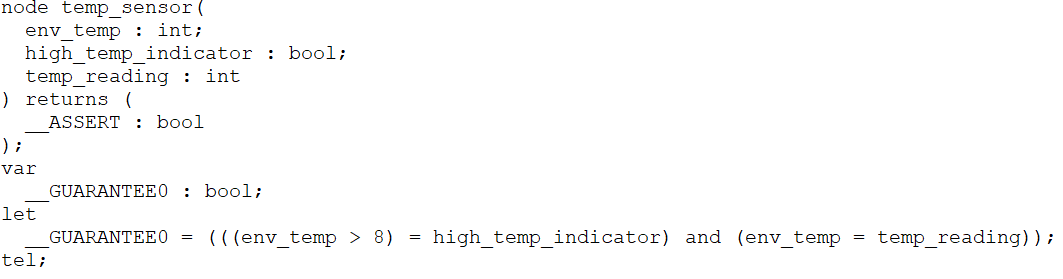
\includegraphics[width=1.0\textwidth]{images/lustreTwoGuar.PNG}
\caption{Temp Sensor With Original Guarantee} \label{fig:lustreOneGuar}
\end{center}
\end{figure} 
Given the property \texttt{((env\_temp $>$ 8) $=$ sensor\_high)}, in the first case, \texttt{GUARANTEE0} is an MIVC for the safety property. Since both the fault defined on the temperature indicator and the fault defined on the temperature reading output affect \texttt{GUARANTEE0}, the minimal cut sets contain both faults. 

We then ran JKind on the model using Algorithm~\ref{alg:splitAnd}. The results of the algorithm on the Lustre encoding of the temperature sensor can be seen in Figure~\ref{fig:lustreTwoGuar}. 

\begin{figure}[h!]
\begin{center}
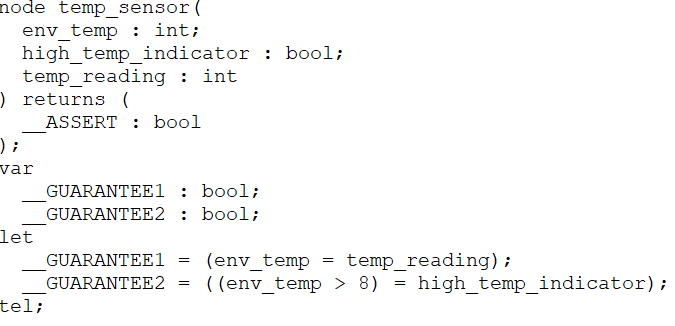
\includegraphics[width=.8\textwidth]{images/lustreOneGuar.PNG}
\caption{Temp Sensor With Modified Guarantees} \label{fig:lustreTwoGuar}
\end{center}
\end{figure} 

 In the second case, only \texttt{GUARANTEE2} is the IVC for the property. The minimal cut sets produced reflected what we expected and show only the high temperature indicator fault for the analysis in Figure~\ref{fig:lustreTwoGuar}. 

While this algorithm is efficient and quite simple, it only catches the low hanging fruit, so to speak. Due to the logical nature of how the Lustre model is analyzed, all guarantees are viewed as a conjunction; therefore, splitting guarantees into new statements only works on the $\land$ operator. This is sufficient for illustration and an initial test into the problem, but cannot provide much decomposition in a general model. 

\subsection{Results of Initial Contractual Refinement}
\label{sec:resultsAND}
The initial contractual refinement was implemented in the safety annex and performed over the AGREE nominal guarantees. We tested the 18 AADL models used in Section~\ref{} and compared the timing results of the generation of minimal cut sets without granular refinement and with this algorithm. The results can be seen in Figure~\ref{}. 

In most cases, the time of analysis is not increased. This is partially due to the size of the model in terms of the number of contracts, but also due to the specifications themselves; if a model does not contain conjunctive contracts, no refinement occurs and the number of contracts in the model remains constant between both forms of analysis. The last three models of the set are all variations on the wheel brake system described in Section~\ref{sec:wbs}. The complexity of the contracts and number of conjunctions used is much higher than the other models and can be seen in the total analysis time using this refinement approach. \danielle{Make figure, finish discussion.}